\chapter{Een identiteit bewijzen}
\label{ch:identiteit-bewijzen}

Het verzekeren van identiteit, oftewel authenticatie, is een proces dat we elke
dag gebruiken. Ieder wachtwoord, zij het om aan te melden op onze computer,
on mobiel apparaat te ontgrendelen of de deur met een sleutel opendoen, dient om onze identitiet te bewijzen. Deze gevallen zijn echter
een voorbeeld van authenticatie met een bekend endpoint en deze zijn vaak
ontoereikend. Een voorbeeld hiervan is wanneer we surfen op het internet en ons
moeten verzekeren van de identiteit van een website. We willen namelijk niet dat
een website ongemerkt zich voordoet als een online banking portaal. Hiervoor
bestaan digitale certificaten die de identiteit van de website bevestigen. Deze
certificaten werken aan de hand van een \gls{PKI},
en worden beheerd door certificaatautoriteiten.

\section{Public key infrastructure}
\label{sec:public-key-infrastructure}

Het doel van een public key infrastructure is systeem van procedures om digitale
certificaten te distribueren, valideren, creëren, opslaan en terugtrekken. De
\gls{PKI} maakt digitale certificaten die een publieke sleutel linken aan een
entiteit. Verder is een \gls{PKI} ook verantwoordelijk voor het terugtrekken van
certificaten indien dit nodig is.

\section{Public key cryptografie}
\label{sec:public-key-cryptografie}

Public key cryptografie is vorm van cryptografie waarbij twee sleutels gebruikt
worden, een private en een publieke. De publieke sleutel, zoals de naam doet
vermoeden is publiekelijk gekend en kan dus door iedereen gezien worden. De
private sleutel moet te allen tijde geheim gehouden worden. Twee communicerende
partijen (A en B) hebben elk hun publieke en private sleutel. In het volgende
voorbeeld gebruiken de veel voorkomende namen (A)lice en (B)ob
\autocite{Rivest1978}.

Als Bob een bericht stuurt naar Alice, zal Bob dit bericht versleutelen met de
publieke sleutel van Alice en dan versturen. Hierna kan enkel Alice haar private
sleutel het bericht decrypteren.

\begin{figure}[H]
	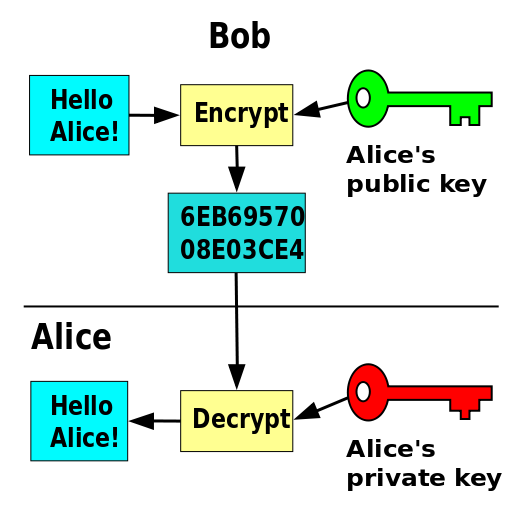
\includegraphics{img/pki-alice-and-bob}
	\centering
	\caption{\gls{PKI} met als voorbeeld Bob die een bericht stuurt naar Alice}
	\label{fig:pki-alice-and-bob}
\end{figure}

Deze toepassing van public key encryption creëert confidentialiteit door het
bericht niet leesbaar te maken voor een 3de partij. Een andere toepassing
hiervan is digitale handtekeningen. Hierbij wordt een bericht ondertekend door
de zender en kan de ontvanger de handtekening controleren aan de hand van de
publieke sleutel van de verwachte zender. Als de ontvanger deze handtekening
controleert en de controle slaagt, dan betekent dit dat de verzender toegang had
tot de private sleutel en kan er geconcludeerd worden dat de verzender de
eigenaar is van de publieke sleutel. Hierdoor wordt ook verzekerd dat het
bericht niet aangepast geweest is, sinds validatie van een aangepast bericht
niet zal slagen met de originele handtekening.

Deze vorm van cryptografie is in het algemeen gebaseerd op wiskundige problemen
die nog niet efficiënt kunnen opgelost worden zoals het factoriseren van gehele
getallen. De wiskunde die cryptografie mogelijk maakt ligt echter buiten het
bereik van deze bachelorproef.

\subsection{Compromitatie van een private sleutel}
\label{subsec:comprimitatie-van-een-private-sleutel}
Het compromitteren van een private sleutel leidt tot een algeheel verlies van de
confidentialiteit van alle toekomstige en ooit versleutelde berichten. Het maakt
het ook mogelijk om zowel handtekeningen als versleutelde berichten aan te maken
in naam van de identiteit wiens sleutel werd verloren. Dit maakt het des te
belangrijker om een systeem te hebben waarin sleutels kunnen worden
geïnvalideerd.

\subsection{Verlies van een private sleutel}
\label{subsec:verlies-van-een-private-sleutel}
Het verliezen van een private sleutel verschilt in compromitatie in de zin dat
de sleutel niet in handen is van een partij met potentiële kwaardaardige
bedoelingen. Hierbij is enkel de mogelijkheid om te handtekeningen en berichten,
die geëncrypteerd zijn met de publieke sleutel, te decrypteren, verloren.
